\section{The Android Sound Stack}\label{sec:androidaudiostack}
In this section we describe the Android sound stack as per the official \textit{Android Open Source Program}\cite{sound_stack}.
We look into the Android sound stack to identify parts of the sound stack,
which can have an effect on the sound latency and furthermore identify parts of the sound stack which can be customized to cater our needs.

We go through the stack and briefly describe the different parts.
During the description we point out the parts of the stack which can be relevant in the design of our system.

The Android sound stack is all the different components which makes up the sound system on Android devices.
On \cref{fig:sound_stack} the full sound stack can be seen for a standard Android system.

\subsubsection*{Application Framework}
On the top of the stack is the application framework.
This is the framework an app, coded in Java, uses for sound.
For instance the \code{android.media.*} frameworks, which are a part of the application framework.
When using the application framework, the Android \ac{SDK} is used.

Using the application framework can potentially be slower, compared to the native framework.
This is caused by the fact that the application framework is higher up the stack than the native framework thus further away from the ``bare metal''.
Therefore it is important to consider if the application framework should be used,
since it is the only thing the Java app interfaces with directly,
and the choice of framework can have big consequences on the performance and functionality of the app.

\subsubsection*{JNI}
Below the Application Framework in the stack is the \ac{JNI}.
The \ac{JNI} makes it possible for Java code to call and be called by the native applications\cite{jni}.

\subsubsection*{Native Framework}
The native framework is below the \ac{JNI} in the stack and used for implementing apps which run natively on the system.
To run natively on the system an app can be written in C++.
When writing apps for the native framework, the Android \ac{NDK} is used.

Using the native framework can give improved performance compared to the application framework used with Java\cite{nat_perf_2}.
This can result in lower latency, and could potential be an advantage when dealing with synchronization of audio.
Therefore the native framework should be considered when designing an app to solve the problem statement.

\subsubsection*{Binder Inter-process Communication Proxies}
One level down in the stack, below the native framework, are the Binder \ac{IPC} Proxies.
The purpose of the Binder \ac{IPC} Proxies is to facilitate communication over process boundaries.

\subsubsection*{Media Server}
Below the Binder \ac{IPC} Proxies stack wise, but on \cref{fig:sound_stack} at the right of the native framework, is the media server.
The media server contains the audio services, which is the code that interacts with the \ac{HAL}.
The \ac{HAL} is right below the media server, in the sound stack.
The sound server implementation on Android is called AudioFlinger, and runs within the media server process\cite{audioflinger}.

It is possible to change the media server,
for instance an example is given where changing from AudioFlinger, to a media server called Superpowered Media Server for Android\footnote{\url{http://superpowered.com/}}, saved $8 ms$ on the round-trip latency on a HTC Nexus 9\cite{superpowered_8ms}.
The round-trip latency is the time it takes sound to be recorded by the microphone,
travel through the audio stack to the user application and then back through the stack to the speakers~\cite{superpowered_8ms}.
Since audio latency can be reduced by making changes to the media server,
then it should be taken into account when designing an app to solve the problem statement.

\subsubsection*{Hardware Abstraction Layer}
Below the Media Server in the stack is the \ac{HAL}.
The \ac{HAL} is the standard interface between the audio services and the audio driver.
The \ac{HAL} is driver-agnostic, which means it can work with any drivers without making any special adaptations.

\subsubsection*{Linux Kernel}
At the bottom of the stack is the Linux Kernel, where the audio driver resides.
Different audio drivers exist, e.g. \ac{ALSA} and \ac{OSS}, which are made for Linux but custom drivers are also available.

Since the \ac{HAL} is driver-agnostic, then the audio driver can be changed without having to alter the \ac{HAL}.
Several audio drivers exist for Android, e.g. ``Voodoo Sound'' or ``ViPER4Android音效FX v2版'',
but it is also possible to make a custom audio driver\cite{voodoo_sound, viper4_android}.
Therefore the sound driver in the Linux kernel should be considered as well, in the design of an app to solve the problem statement.
\begin{figure}[!bht]
    \centering
    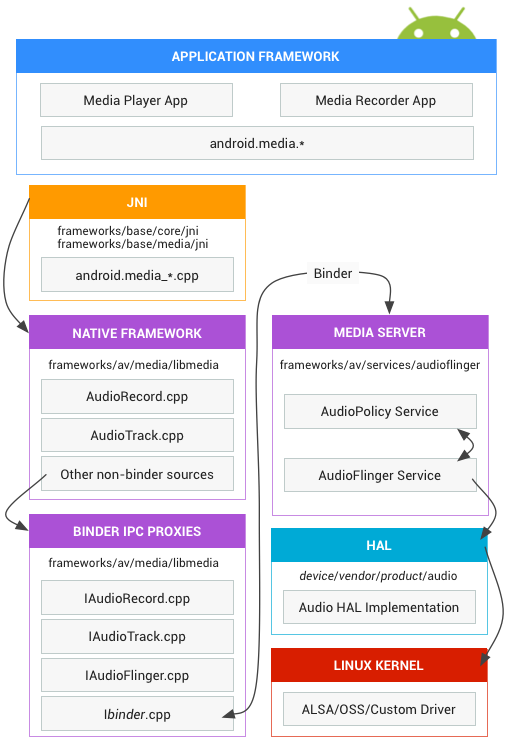
\includegraphics[width=0.5\textwidth]{img/sound_stack.png}
    \caption{The Android audio stack\cite{sound_stack}.}
    \label{fig:sound_stack}
\end{figure}

\subsection{Summary}
The sound stack on Android has several layers, which sound have to go through,
where each layer can potentially add latency to the sound.
Some of these layers are more relevant for this project than others, since we can affect them,
especially the application framework, native framework, media server and Linux kernel.
These layers should be considered when an app to solve the problem statement is designed.


